\chapter{Design}\label{chap:design}

This chapter describes the design of core components of the system.

The architecture of the system is presented in \Cref{sec:architecture}.
\Cref{sec:detecting-points} describes the approach we took for detecting if the user is pointing.
In order to determine which device should perform the action, 
without a line of sight requirement, 
we need to know the \emph{indoor position} of the user, 
the position of the device(s) and the heading of the user. 
We will discuss how we get the location of the devices and the user in \Cref{sec:design:indoor-positioning}.
In \Cref{sec:design:indoor-positioning} we discuss the differences between region monitoring and ranging, 
in regards to indoor positioning. 
Furthermore we propose a design for configuring rooms for indoor positioning.
At last, as described in \Cref{sec:smarthomes}, 
we need a smart hub to allow communication between the different devices, 
including the wearable, to be able to perform actions on the devices. 
We design a server to hold information about the locations of devices,
and to communicate with a smart hub in \Cref{sec:serverdesign}. 

Our approach to a solution thus requires accurate indoor position, 
a wrist-worn wearable that can recognize gestures, 
and a hub for interoperability between the wearable and the smart devices. 

\section{Architecture}\label{sec:architecture}
The system consists of three layers as illustrated in \Cref{fig:architecture}. 
Each layer can communicate with the layer below and above it if they exist.

The first layer consist of the wearable device and the smartphone. 
The two may be tightly coupled as some wearable watches, 
for example the Apple Watch, relies heavily on the phone. 
The two devices are responsible for listening to new movement data from the wearable, 
\eg new data from the accelerometer and the magnetometer.
The movement data is used for recognizing gestures, 
and the magnetometer data is used for determining direction, 
such that we are able to determine what devices are being pointed at. 
The topmost layer is also responsible for communicating with the beacons, 
in order to retrieve the position of the user, 
and possibly the position of the devices the user can control. 

The topmost layer communicates with a central server developed specifically for this project. 
The server is responsible for storing positions of the smart devices, 
as well as receiving actions, based on interpreted gestures, from the wearable device.
Whenever the wearable device recognizes a gesture, 
the wearable devices sends an action and a device ID to the server.
The server then relays this request to a smart hub. 

The smart hub is responsible for managing the devices that can be controlled using gestures. 
The smart execute the request received from the server, 
on the appropriate smart device. 

When utilizing a smart hub, users must install a hub in their home. 
The hub communicates with the users devices, \eg bulbs, locks and thermostats. 
For privacy reasons, it may be interesting to move the logic of the server to the smart hubs in the users home. 
This would also remove a layer in the architecture, simplifying it.

\begin{figure}[H]
  \centering
  \begin{tikzpicture}
    \node[anchor=center] at (-0.8,0.5) {(1)};
    \node[anchor=center] at (-0.8,-1.5) {(2)};
    \node[anchor=center] at (-0.8,-4) {(3)};
    
    \node[anchor=center] at (2.5,0.5) {Wearable Device};
    \node[anchor=center] at (7.5,0.5) {Mobile Device};
    \draw[thick] (0,0) rectangle (10,1);
    \draw[thick, dashed] (5,0) -- (5,1);
    \draw[thick,->] (10.85,0.5) -- (10.15,0.5);
    \draw[thick] (11,0) rectangle (13,1) node[pos=.5] {Beacons};
    
    \draw[thick] (0,-1) rectangle (10,-2) node[pos=.5] {Server};
    \draw[thick,<->] (5,-0.15) -- (5,-0.85);
    
    \node[anchor=center] at (1.2,-3.4) {SmartThings};
    \draw[thick] (0,-3) rectangle (10,-5);
    \draw[thick,<->] (5,-2.15) -- (5,-2.85);
    \draw[thick] (0.2,-3.8) rectangle (2.7,-4.8) node[pos=.5] (bulb) {Bulb};
    \draw[thick] (2.9,-3.8) rectangle (5.4,-4.8) node[pos=.5] (lock) {Lock};
    \draw[thick] (7.3,-3.8) rectangle (9.8,-4.8) node[pos=.5] (door) {Thermostat};
    \node at ($(lock)!.5!(door)$) {\ldots};
\end{tikzpicture}
  \caption{Architecture of the system.}
  \label{fig:architecture}
\end{figure}

The following components are involved in the architecture:
\begin{description}
    \item[Werable Device] Recognizes gestures and ensures actions are sent. Not included in the implemented prototypes; gesture recognition is performed on a smartphone in out implementation. For more information on gesture recognition, see \Cref{sec:gesturerecognition}.
    \item[Smartphone] Responsible for performing indoor positioning using the beacons. Possibly serves as a medium of communication between the wearable and the server, as some wearable devices require a coupled smartphone.
    \item[Beacons] Utilized for indoor positioning. For more information on this see \Cref{sec:designindoorlocation}.
    \item[Server] A medium of communication between layer (1) and layer (3). For more information about the server, see \Cref{sec:serverdesign}.
    \item[Smart Hub] The hub responsible for communicating with the smart devices. For more information on the smart hub, see \Cref{sec:designsmarthub}.
\end{description}

In the architecture presented in \Cref{fig:architecture}, 
the server is separated from the smart hub. 
In the current prototype, 
the components are physically separated. 
In practice it makes sense to bundle the two components together, 
and keep a virtual separation. 
Based on the current solution, 
the user must install both a server and a smart hub in his home. 
Bundling the two together eases the installation, 
as only a single component will need to be installed, 
and configured by the user.

One way of bundling the two components, 
is to extend the smart hub with the capabilities of the server. 
This is possible if the smart hub solution is open sourced, 
and we have access to the entire implementation. 
Such solution is not possible with other hubs, such as SmartThings.
In order to bundle with such smart hubs, 
the capabilities of our server must be implemented by the company making the smart hub. 


%%% Local Variables:
%%% mode: latex
%%% TeX-master: "../../master"
%%% End:

%!TeX root=../../master.tex
\section{Detecting Points}\label{sec:detecting-points}

Before a user performs a gesture in order to control a smart device, 
he must point at the smart device he desires to control. 

Pointing at a smart device informs the system which device actions should be sent to. This allows multiple devices to share actions and only the device being pointed at, will be receive the action. Configuring multiple devices with the same gesture means that the users can configure fewer gestures as they can be used.

A point is defined as the user holding his phone still for a small period of time. 
An accelerometer can be used to detect if the user holds the device still. 
If there is a low amount of activity on all three axes, 
it is assumed that the user is holding the device in his hand without moving it.

\Cref{fig:point-to-gesture-state-diagram} shows the relationship of a point and a gesture in a state diagram. 
All gestures begin and end with a point. 
When the first point is detected, 
a very short delay is introduced in order for the user to prepare to do the gesture, 
\eg move the position of his hand. 
The delay was added because from testing on our own we found that if there was no delay, the recognition would suddenly begin without the user being prepared, resulting in the first data being invalid and not part of any gesture and ultimately the gesture would not be recognized.
The gesture recognition begins when the delay has passed. 
Gestures are recognized using the previously described \$3 Gesture Recognizer. 
After the gesture has been performed, 
the device must be held still again and the second point is detected. 
The collected gesture data is then analyzed by the \$3 Gesture Recognizer, 
in order to determine which known gesture was performed, if any at all. 
Lastly, the system returns to the initial state and another gesture can be performed.

While performing the gesture, the recognition may timeout. 
The \$3 Gesture Recognizer can recognize gestures for a maximum of four seconds before the recognition is canceled. 
In such case, the system returns to the initial state.

\begin{figure}[h]
\centering
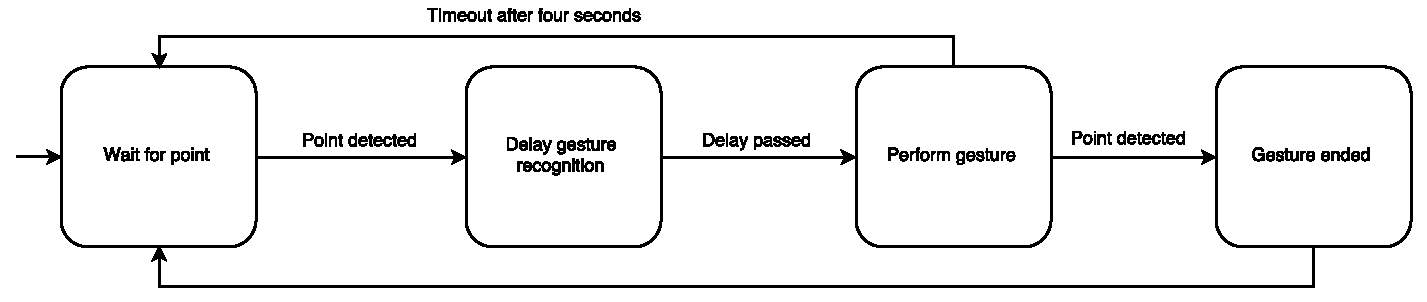
\includegraphics[width=\textwidth]{images/point-to-gesture-state-diagram}
\caption{State diagram showing the relationship between a point and a gesture. A gesture always starts and ends with a point.}
\label{fig:point-to-gesture-state-diagram}
\end{figure}

\subsubsection{Using Accelerometer Data to Detect a Point}

\Cref{fig:pointer} shows screenshots of an application, 
created to experiment with data from the accelerometer. 
The figure shows graphs of measurements made while the device was lying on a table (\Cref{fig:pointer:table}), 
the user was pointing with the device in his hand (\Cref{fig:pointer:hand}), 
and while the user was walking with the device in his hand (\Cref{fig:pointer:walk}).
We measure this so that we do not recognize a device laying still on a table, 
as a user pointing.
 
The $x$-, $y$- and $z$-values are measured in radians per second. 
The $y$-axis of the graph spans from \num{-5} to num{5}. 
The graphs shows that there are small, 
but measurable differences between the measurements made when the device is lying on the table,
and when the user is pointing with the device. 
This allows us to distinguish between the two scenarios, 
and disregard measurements made when the device is lying on the table. 

Furthermore the graphs clearly shows that there is a measurable difference between the values read when a user is pointing with a device, 
and walking with the device in his hand. 
Based on this small experiment, 
we can conclude that the accelerometer data can be used to determine if a user is pointing with a device.

\begin{figure}[!htb]%
    \centering
    \subbottom[Table]{\label{fig:pointer:table}
        \frame{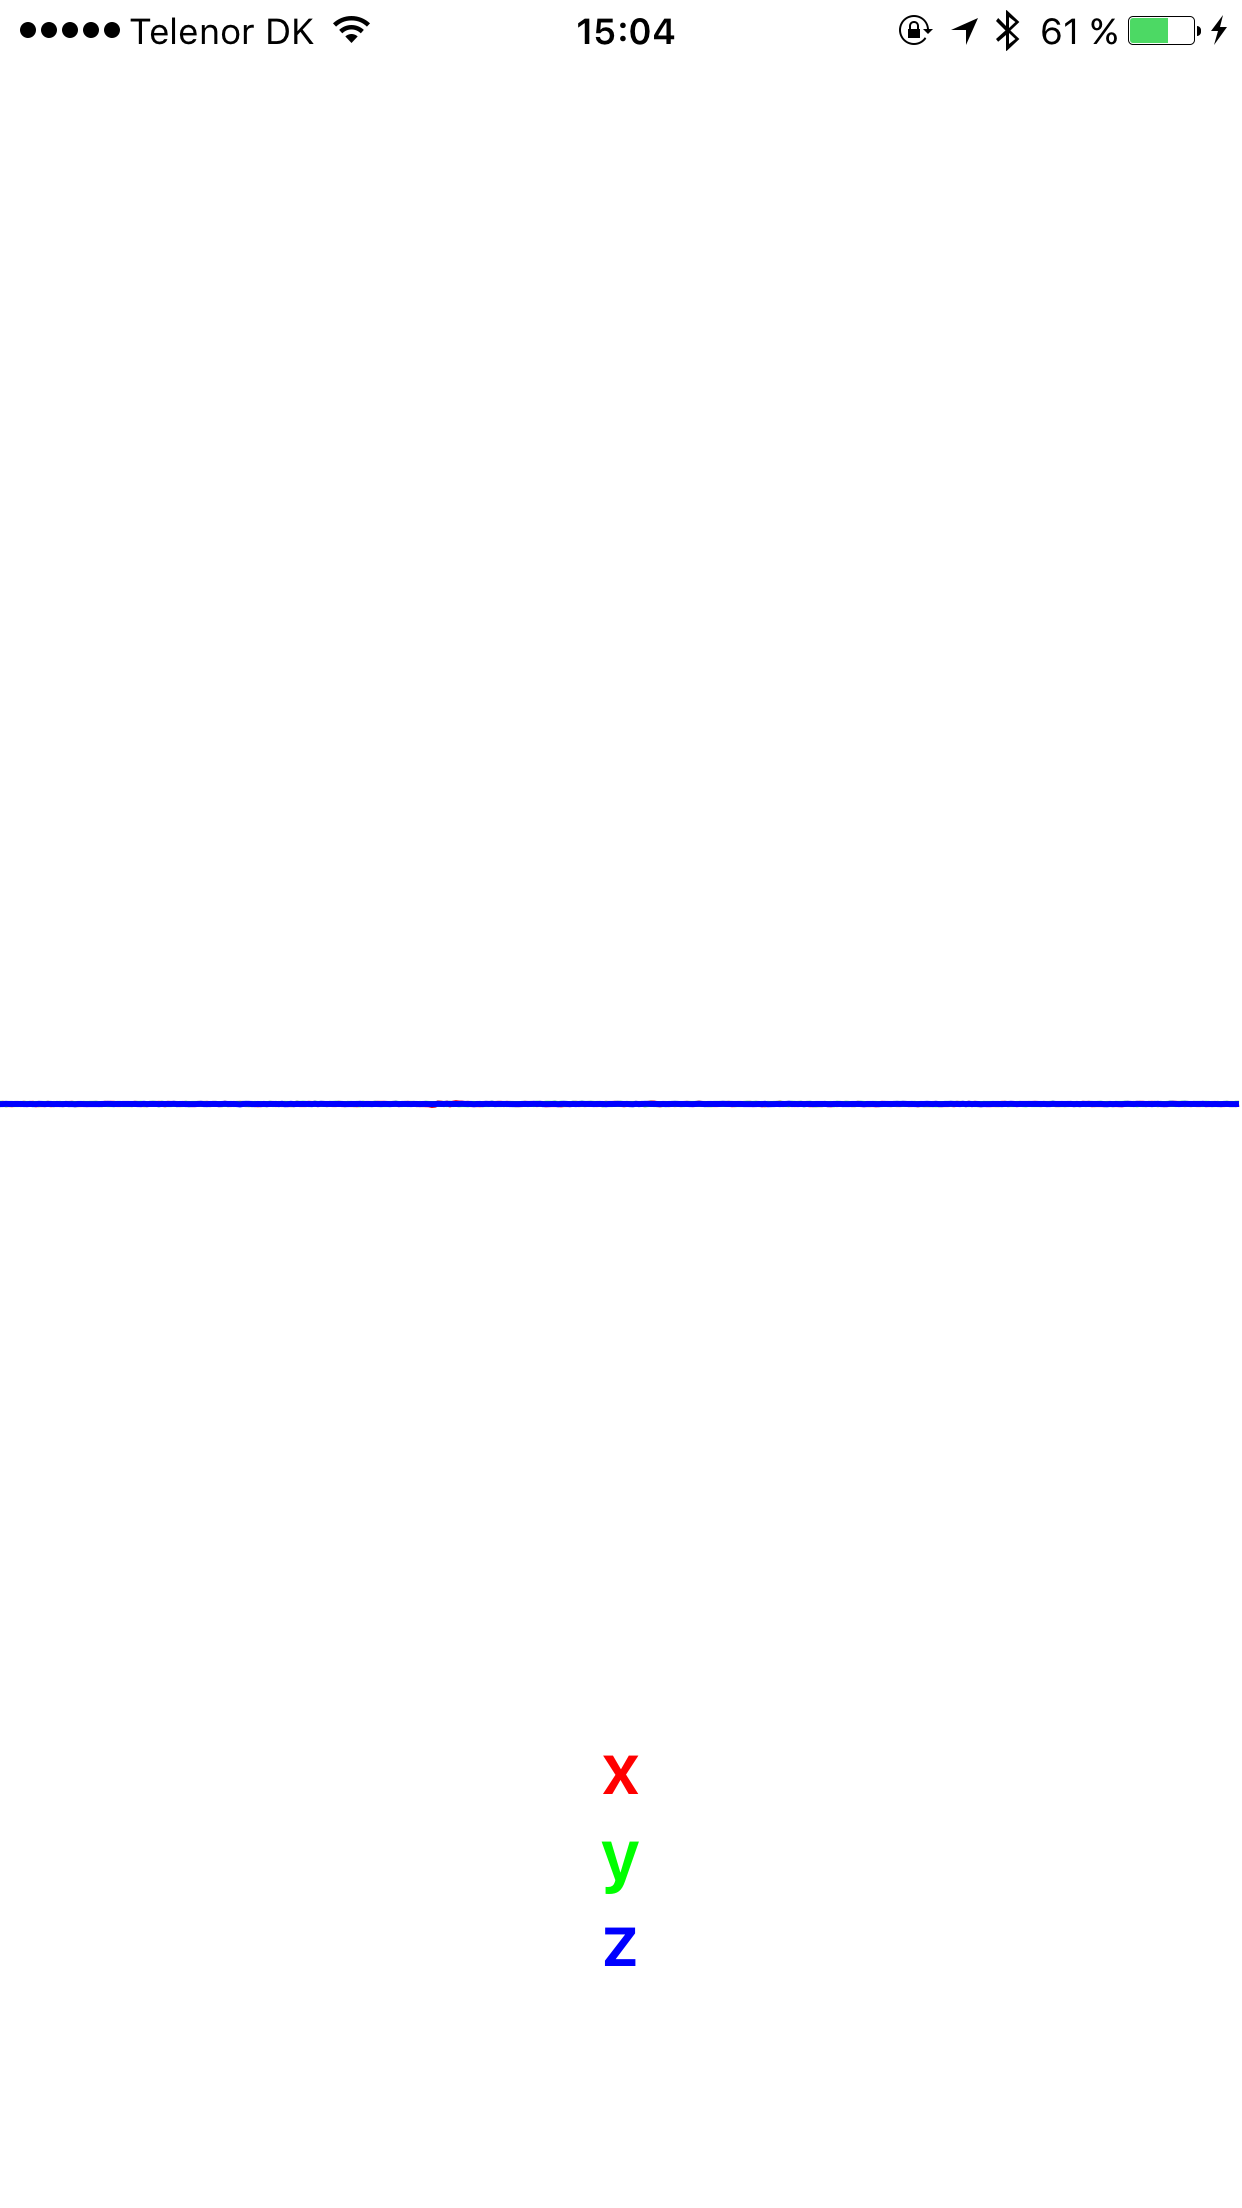
\includegraphics[width=0.3\textwidth]{images/pointer-table}}
    }
    \subbottom[Hand]{\label{fig:pointer:hand}
        \frame{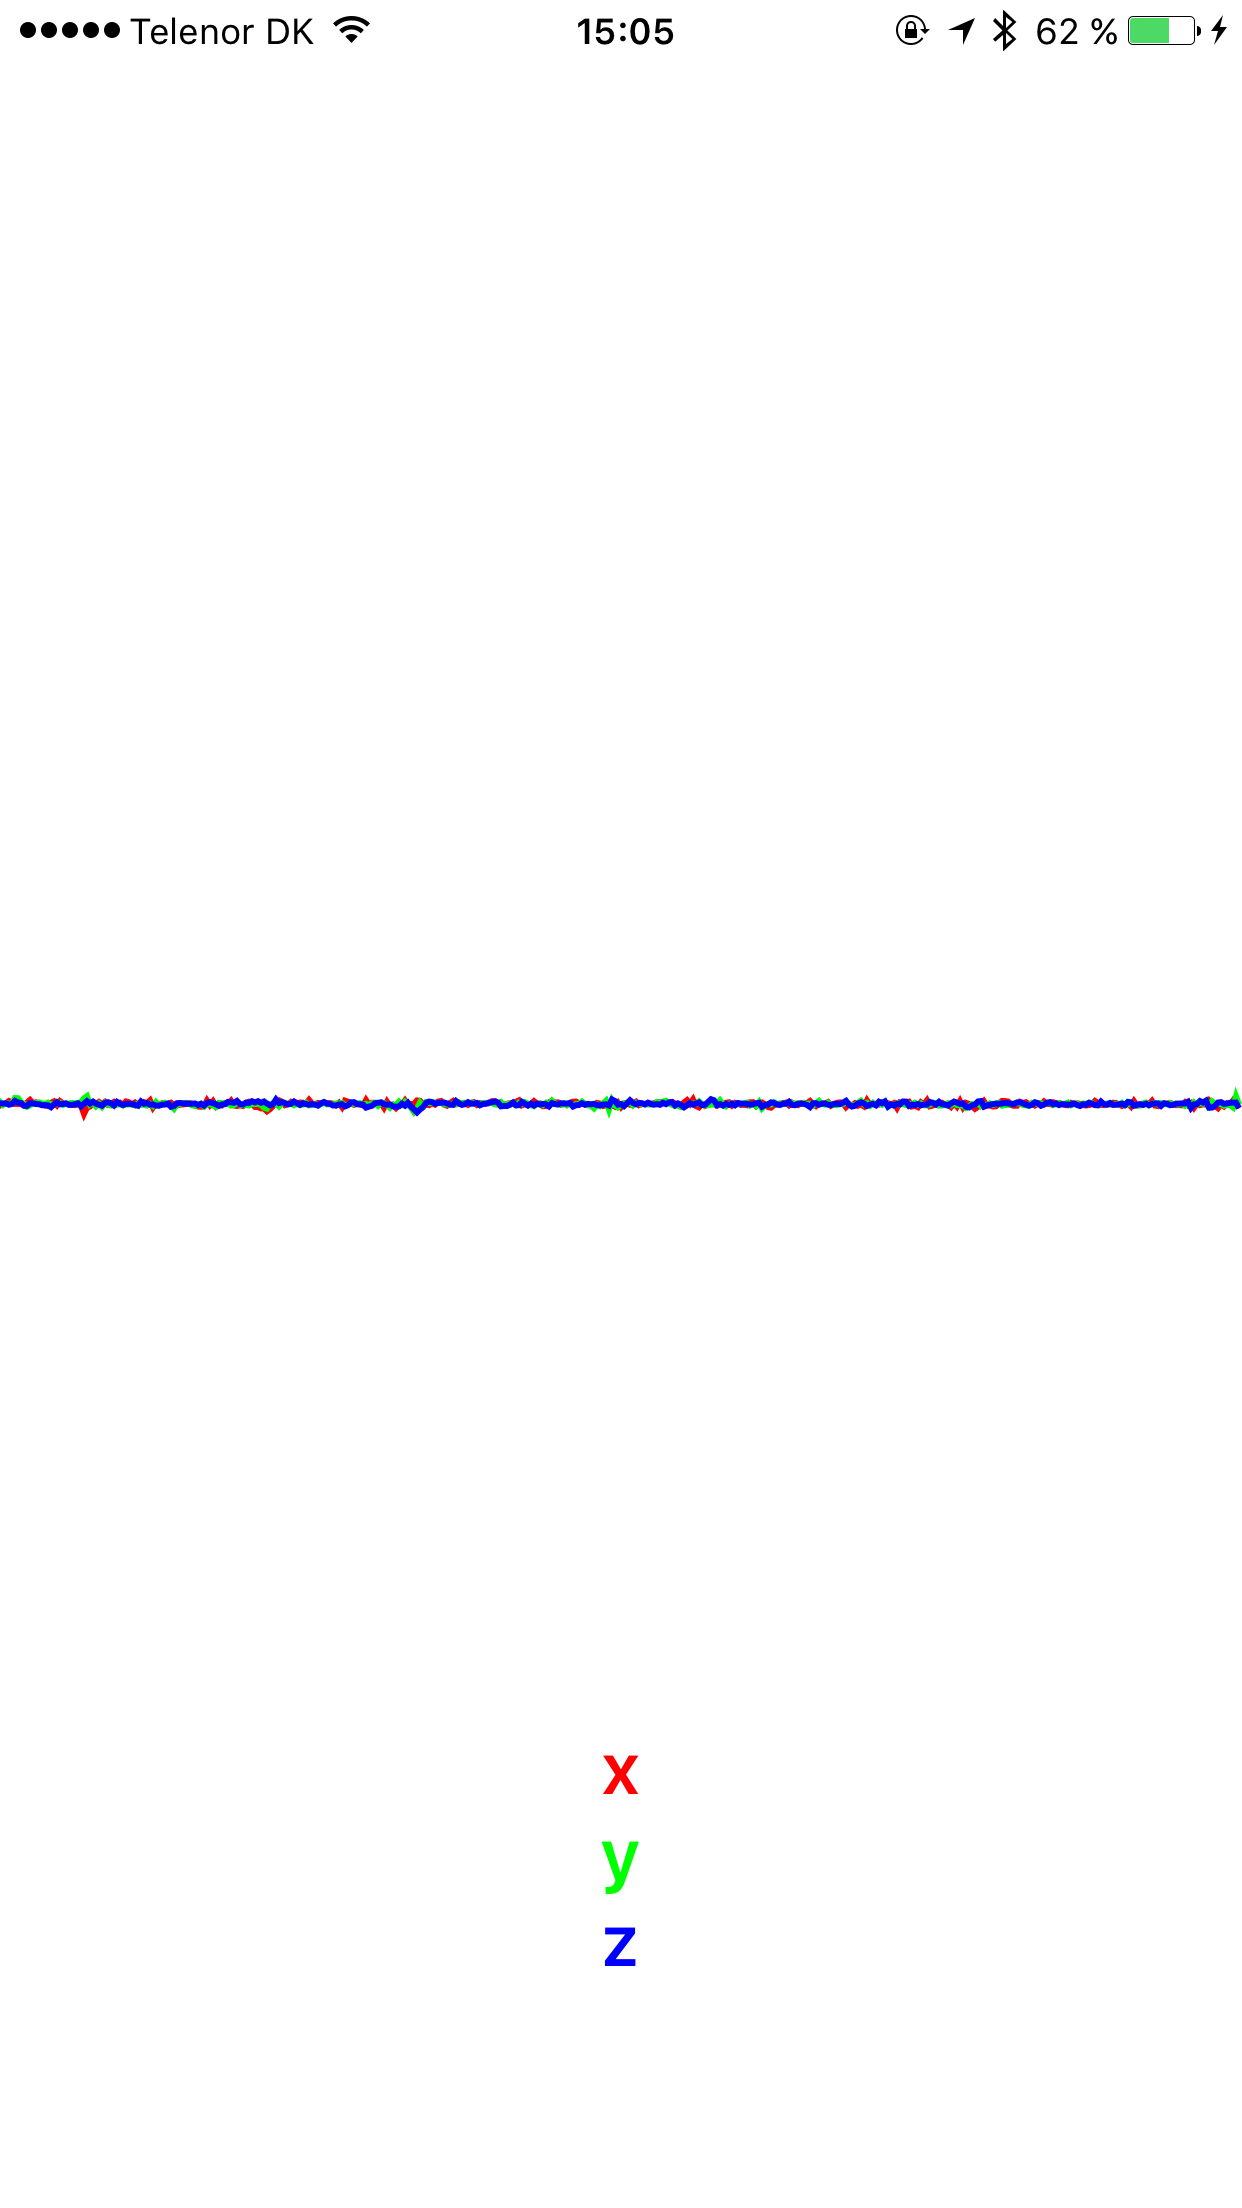
\includegraphics[width=0.3\textwidth]{images/pointer-hand}}
    }
    \subbottom[Walk]{\label{fig:pointer:walk}
        \frame{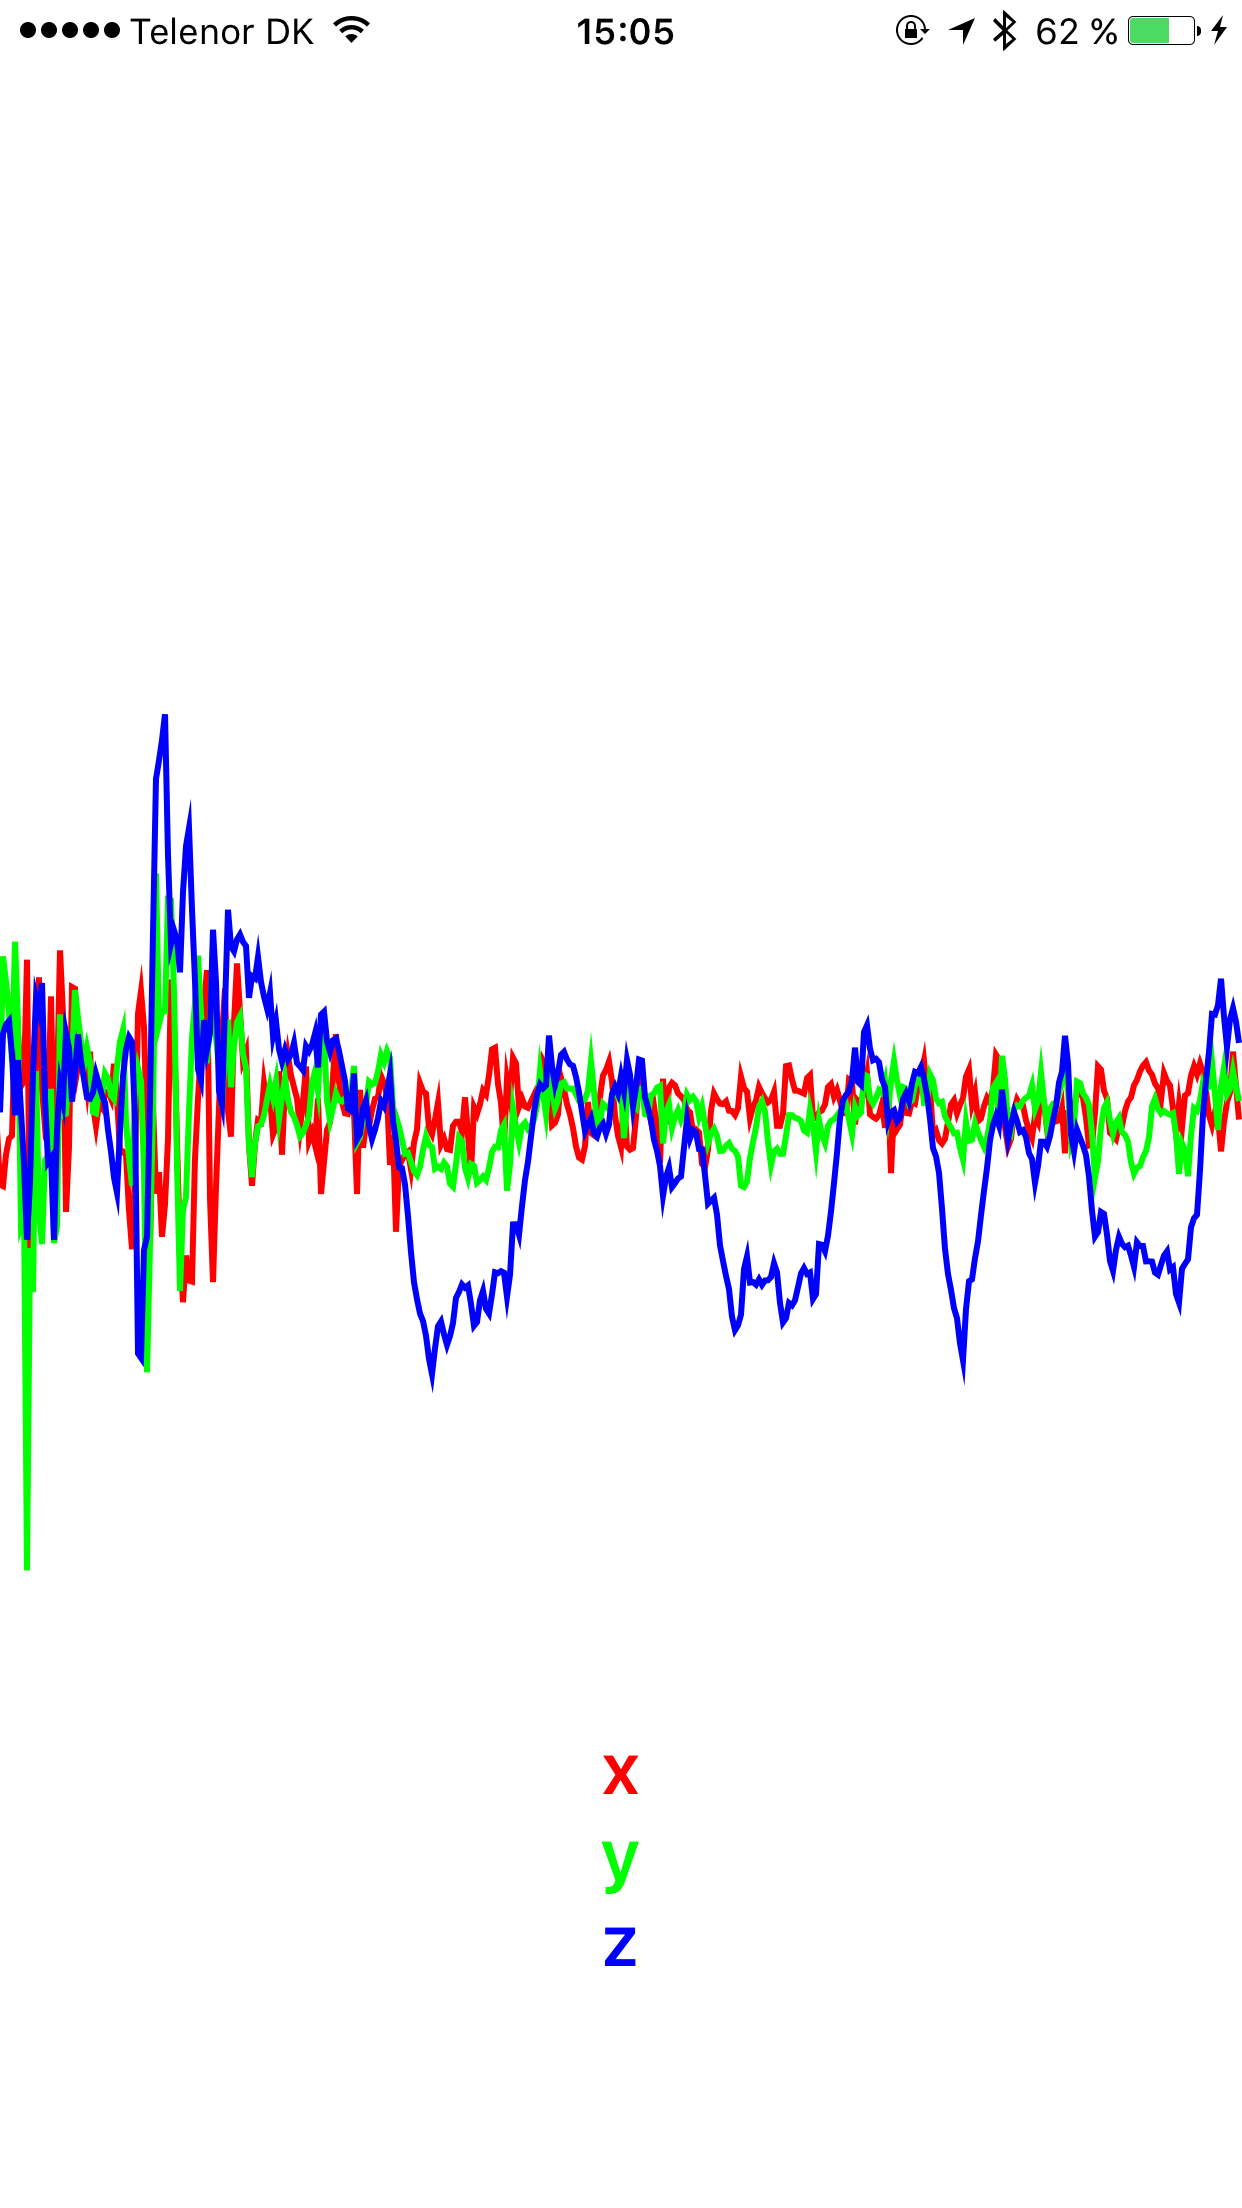
\includegraphics[width=0.3\textwidth]{images/pointer-walk}}
    }
    \caption{Screenshots of application created to experiment with data from the accelerometer. Leftmost screenshot shows graph of measurements made when the device lies on a table. The middle image shows graph of measurements made while pointing with the device. Rightmost screenshot shows graph of measurements made while the user was walking with the device in his hand.}
    \label{fig:pointer}
\end{figure}

\subsubsection{Detecting Points using PointDetector}

Part of the gesture recognition involves detecting if a user points. 
In order to limit the scope for the initial prototypes of the solution, 
we limit the context in which a point is detected, 
to a user walking with the phone in his hand, 
then stopping up to point at an actuator with the phone.

The \texttt{PointDetector} class receives data from the accelerometer data, 
and based on the data determines if a user points with the device. 
When a user points with the device, 
an instance of the class will inform a listener.

The state diagram in \Cref{fig:pointdetector-state-diagram} illustrates the internals of the \texttt{PointDetector} class. 
When instantiated, the object will not be detecting, 
\ie it will not be receiving accelerometer data. 
After the instantiation, the instance can begin detecting. 
The detection can be stopped at any time.

When detecting, the \texttt{PointDetector} will wait for the first set of data from the accelerometer, 
that indicates that the user is pointing. 
When the data is received, 
the object will enter the \textit{Sampling} state, 
in which it continuously checks data from the accelerometer, 
to determine if a set of data indicates a point. 
If the data indicates a point, 
both the \emph{point sample count} and the \emph{total sample count} will be incremented. 
If the data does not indicate a point, 
only the total sample count will be incremented.
%Thalley: Beskrivelse af de her sample counts bør nok ligge heroppe. Kunne ikke lige finde en pæn måde at gøre det på selv.

At the same time the detector enters the sampling state, 
it will start a timer that runs for a number of seconds. 
When the time has passed, 
the detector will leave the sampling state, 
and determine if the result of the sampling, 
indicates that the user is pointing. 

The sampling phase is necessary in order to avoid ``outliers'' in the data, 
\ie anomalies in the sensor data. 
The accelerometer continuously delivers data, 
and a single data set may indicate that the user is pointing. 
However, it may not be the users intention to point at all. 
It may be that he just held the device very still for a short moment.

In order to determine if the result of the sampling phase indicates a point, 
the detector investigates the relation between the point sample count, $p$, 
and the total sample count, $t$. 
If $p/t \geq c$, where $c$ is the necessary percentage of samples that must indicate a point, 
then the detector can conclude that the sample is indeed a point.

After the sampling phase has concluded, 
the detector will wait for a new data set from the accelerometer that indicates a point.

An accelerometer delivers an $x$-, $y$- and $z$-acceleration. 
Determining if a data set indicates a point is a matter of checking if the three values fits within some threshold, $h$. 
In order to check if the phone is lying still on a table, 
the values must be checked against another threshold, $g$. Note that $g < h$.

\begin{figure}
\centering
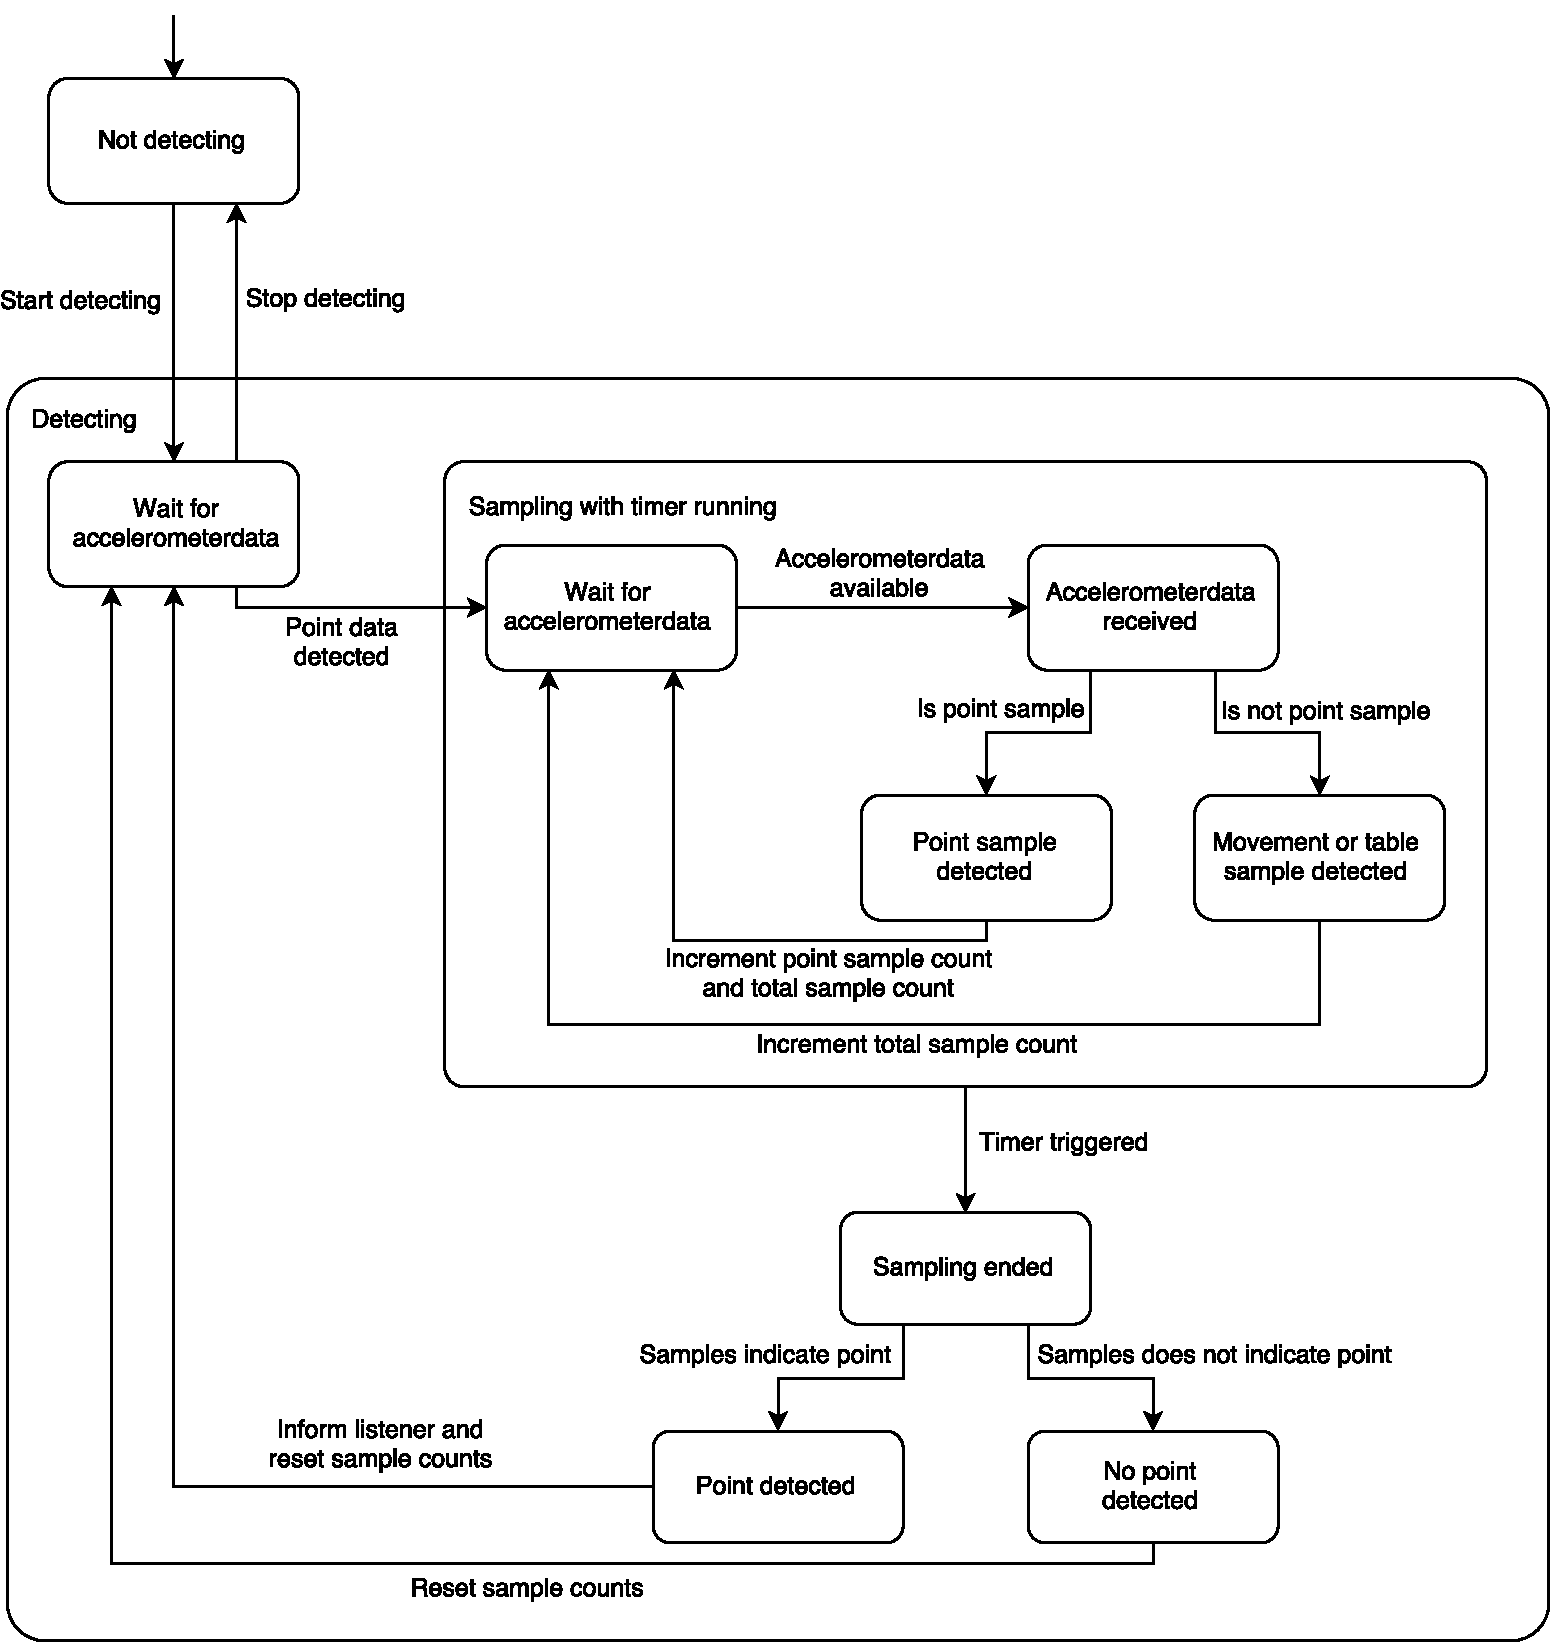
\includegraphics[width=\textwidth]{images/point-detector-state-diagram}
\caption{State diagram showing the states the \texttt{PointDetector} class can be in.}
\label{fig:pointdetector-state-diagram}
\end{figure}

The following pseudo code checks if a data set from the accelerometer indicates a point. 
\texttt{DataFitsWithinThreshold} takes the data from the accelerometer and a threshold $t$. \\
The function returns whether or not all of the $x$-, $y$- and $z$-values in the accelerometer data fits within the threshold.

\begin{algorithm}
  \begin{algorithmic}
    \Function{DataFitsWithinThreshold}{$data$, $t$}
      \State \Return $data.x \leq t \And data.x \geq -t \And data.y \leq t \And data.y \geq -t \And data.z \leq t \And data.z \geq -t$
    \EndFunction
  \end{algorithmic}
\end{algorithm}

The function \texttt{AccelerometerDataIndicatesPoint} takes data from the accelerometer data, 
and checks if the data fits within the threshold $g$, 
indicating that the data comes from a device lying on the table. 
If the data fits within $g$, 
the function returns false. 
If the data does not fit within the threshold $g$, the function checks if the data fits within the threshold $h$ and returns the result of the check as a boolean value. $h$ is some small number that represents an approximate of the acceleration of the device when the user points with it.

\begin{algorithm}
  \begin{algorithmic}
    \Function{AccelerometerDataIndicatesPoint}{$data$}
    \If{\Call{DataFitsWithinThreshold}{data, g}}
    \State \Return \texttt{false}
    \Else
    \State \Return \Call{DataFitsWithinThreshold}{data, h}
    \EndIf
    \EndFunction
  \end{algorithmic}
\end{algorithm}

\Cref{fig:pointdetector-uml} shows an example of the attributes and operations the \texttt{PointDetector} may have. 
Most of the attributes and operations should be self-explanatory but some may need a short description.

\begin{itemize}
  \item \texttt{pointingDuration} specifies the duration of the timer registered when entering the sampling phase.
  \item \texttt{pointingSampleFrequency} corresponds to $c$, the percentage of samples that must indicate a point.
  \item \texttt{pointingThreshold} corresponds to $h$, the threshold of data when determining if the device is lying on the table.
  \item \texttt{tableThreshold} corresponds to $g$, the threshold of data when determining if the device is being pointed with.
  \item \texttt{pointDetectedCallback} is a closure called when a point is detected.
\end{itemize}

By trial and error we found the following thresholds to be suitable:

\begin{itemize}
\item \texttt{pointingDuration} = 0.5
\item \texttt{pointingSampleFrequency} = 0.5
\item \texttt{pointingThreshold} = 0.05
\item \texttt{tableThreshold} = 0.005
\end{itemize}

The thresholds were determined by adjusting the values, 
until an acceptable behavior was achieved. 
No systematic experimentation of the values were performed, 
as we have a hypothesis that the values can be calibrated for each user. 
For example, we found that \texttt{pointingThreshold} to be dependent of the user. 
It depends on how much the user shakes, 
when trying to hold his hand still. 
A solution is to use a value higher than the values measured when he is holding his hand still.
However, the lower the threshold is, 
the better we can detect a point.

\begin{figure}
  \centering
  \begin{tikzpicture} 
    \umlclass[x=0,y=0]{PointDetector}{
    +/- isDetecting: Bool\\
    - isSampling: Bool\\
    - pointingDuration: Float\\
    - pointingSampleFrequency: Float\\
    - pointingThreshold: Float\\
    - tableThreshold: Float\\
    - samplingTimer: Timer\\
    - pointingSampleCount: Int\\
    - totalSampleCount: Int\\
    - pointDetectedCallback: Closure
    }{
    + beginDetecting()\\
    + endDetecting()\\
    - didReceiveAccelerometerData(data: AccelerometerData)\\
    - accelerometerDataIndicatesPoint(data: AccelerometerData): Bool\\
    - dataFitsWithinThreshold(data: AccelerometerData, threshold: Double): Bool\\
    - samplingTimerTriggered()
    } 
  \end{tikzpicture}
  \caption{Class diagram of the \texttt{PointDetector} class.}
  \label{fig:pointdetector-uml}
\end{figure}

%%% Local Variables:
%%% mode: latex
%%% TeX-master: "../../master"
%%% TeX-command-extra-options: "-shell-escape"
%%% End:

\section{Indoor Positioning}
\label{sec:design:indoor-positioning}

There are two distinct ways of positioning a user, 
when using the iBeacon protocol \cite{estimote:monitoring-ranging}.

\begin{itemize}
\item Region monitoring is performed to check, if a user enters or leaves a specific region. A region is a geofence, \ie a virtual perimeter around some location. A region can be used to check, if a user arrives or leaves his house, his workplace or if he is near a shop encapsulated in a geofence. Regions are useful for performing simple home automation, \eg turn the lights on when the user arrives at home, and turn them off when they leave.
\item Ranging is more granular than region monitoring, and is used to continuously retrieve the set of beacons in range, along with an estimated distance to them, based on the signal strengths. Ranging is used to get a granular user position.
\end{itemize}

We use ranging as we are interested in a granular and accurate position of the user as
we need to determine his position relative to the smart devices in his home.

According to both Apple and Estimote it is preferred that ranging is only performed, 
while the application is in the foreground, 
\ie the application is on the screen, 
and the user is likely to interact with the application. 
The reason for this is that ranging for beacons can have a negative impact on the battery life, 
whereas the region monitoring does not use as much battery power.

While Apple and Estimote advise against performing beacon ranging in the background, 
it is possible \cite{apple:monitoring-ibeacon,estimote:monitoring-ranging}.

\subsection{Configuration of a Location}

Before indoor positioning can be performed, 
we must configure the location in where we want to perform the positioning in. 
For Estimote, this is done using the \texttt{ESTLocationBuilder} as described in \Cref{sec:indoor-positioning:estimote}. 
The location builder is sufficient from a developers perspective, 
but configuring locations in code is likely not intuitive for the target group. 
Instead we propose an alternative way to configure locations.

As a minimum, Estimote must be configured with the walls of a location, 
as the beacons are attached to a wall. 
We propose a smartphone application in which users can draw the walls in their home, 
using the touchscreen of the phone. 
This requires users to measure the length of the walls in their home, 
and then plot it on their smartphone. 
For improved accuracy users can fine tune the length of walls, 
by selecting a wall and entering the length in centimeters.

Having configured the walls of the room, 
the user needs to configure the locations of each beacon. 
The first thing he must do is to install the beacons on the actual walls, 
\ie not the virtual representation of his home.
Using the smartphone application, the user can drag a virtual beacon into the representation of his home, 
and place it on one of the previously configured walls. 
He should do so for each installed beacon.
%Thalley: Hvad med precision af beacons? Bør man kunne indstille det også?


The Estimote Indoor SDK must know the MAC address of each positioned beacon, 
in order to do the positioning. 
Using Estimote's regular SDK, \ie not the Indoor SDK, 
signal strengths and MAC addresses for all beacons can be retrieved. 
Based on the signal strengths, 
we can determine which beacon the user is closest to, 
and assign its MAC address to the previously positioned beacon. 
This requires the user to walk along the perimeter of the location when configuring the beacons, 
in order to be closer to the relevant beacon than the rest.
%Thalley: Kan det ikke lade sig gøre med Indoor SDK?

Knowing the layout of the room and the positions of the beacons, 
we can start positioning the user, 
and the only thing left is to configure the location of each actuator, 
in order to determine the relative location of the user and the actuator. 
We can utilize the position of the user when configuring the position of each actuator. 
The user can walk to each actuator he desires to add to the system, 
press a button to add it and for further reference provide some information about the actuator, such as a name.

\Cref{fig:configuration-location:add-room} shows a mock up of software that can be used to configure a location. 
Note that this software was not implemented during the project. 

\Cref{fig:configuration-location:add-room:draw} shows the process of drawing the location. 
The user can use the pencil to draw walls, 
and the erase tool to remove entire walls. 
Tapping on the lengths will present a keyboard, 
allowing the user to adjust the lengths. 
Note that the length of the first wall must be specified manually, 
in order to determine relative lengths when the user draws the following walls.
%Thalley: Giver det mening at sige at vi ikke har implementeret dette? Kunne man ikke nævne det i det næste kapitel?

In \Cref{fig:configuration-location:add-room:beacons} the beacon tool is enabled, 
and the pencil tool and eraser tool are disabled. 
The user should position beacons on the walls, 
by dragging a beacon from the bottom onto a wall.

\Cref{fig:configuration-location:add-room:actuators} shows the user walking around placing actuators. 
Actuators are represented by a circle, 
and two has been placed in the image. 
Recently one was placed at the users current location, 
thus a circle has been put around the user. 
Tapping an actuator lets the user add information about the actuator, such as a name. 
Pressing the done button will save the location.

Locations are created and saved using the \texttt{ESTLocationBuilder}. 
Whenever a location is saved, 
it is stored in the Estimote cloud, 
and is available on all the user's devices. 
In order to authenticate an account with Estimote, 
the user must log into Estimote on \url{cloud.estimote.com}, 
create an application, 
and enter the returned application token into the settings of the smartphone application.

\begin{figure}[!htb]%
    \centering
    \subbottom[Drawing a room]{\label{fig:configuration-location:add-room:draw}
        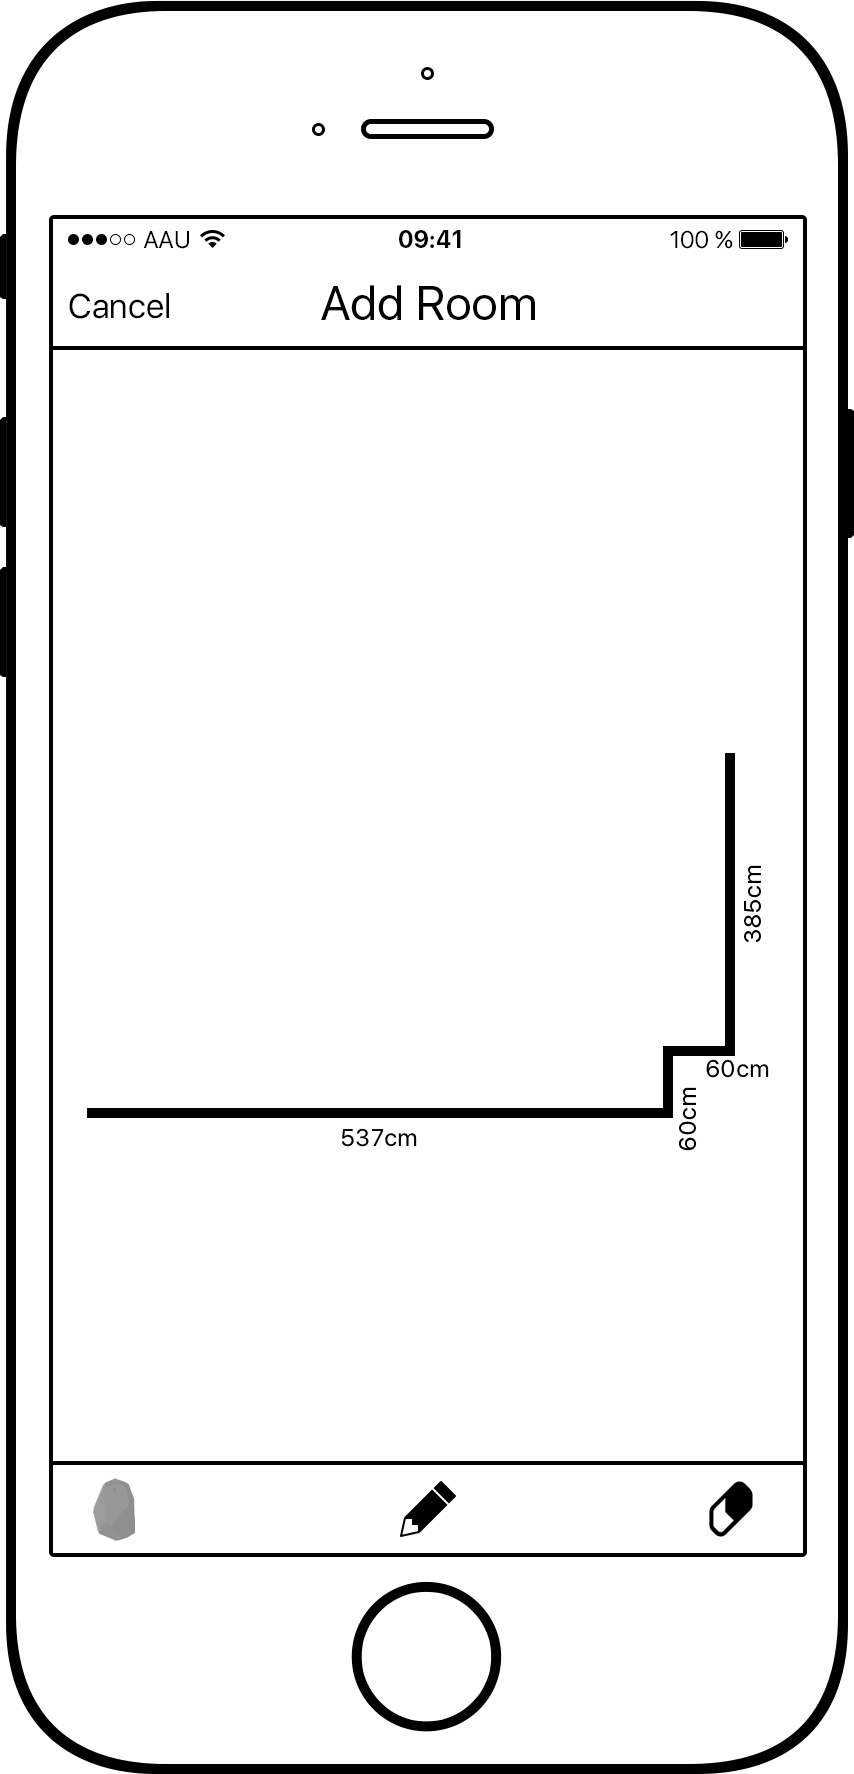
\includegraphics[width=0.3\textwidth]{images/add-room-1}
    }
    \subbottom[Placing beacons]{\label{fig:configuration-location:add-room:beacons}
        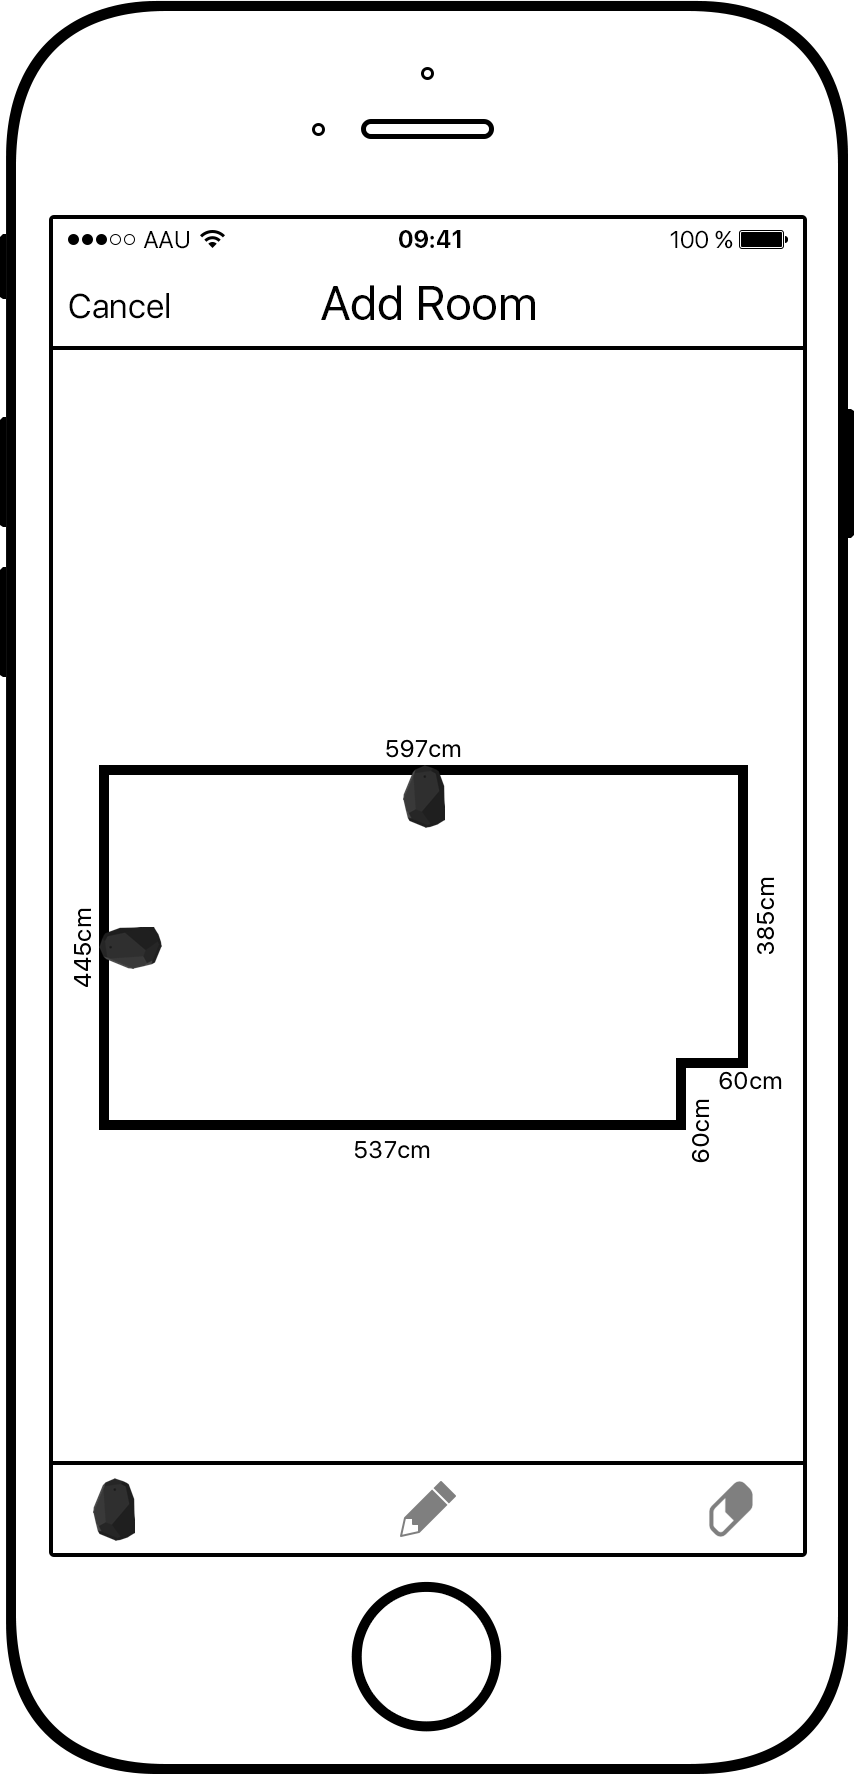
\includegraphics[width=0.3\textwidth]{images/add-room-2}
    }
    \subbottom[Placing actuators]{\label{fig:configuration-location:add-room:actuators}
        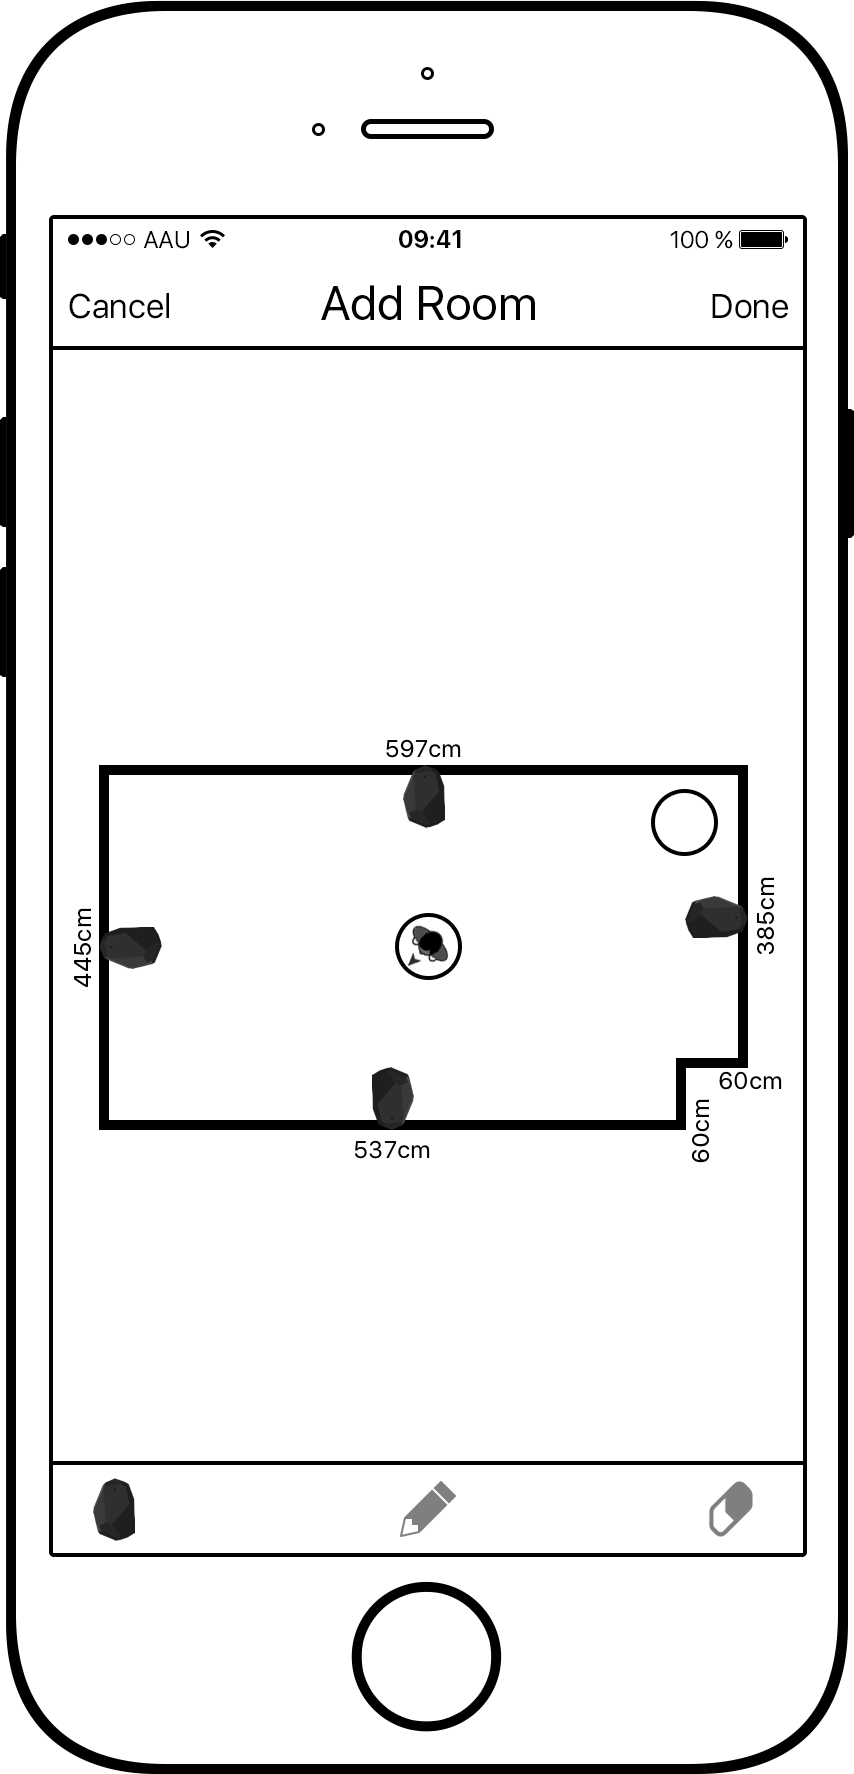
\includegraphics[width=0.3\textwidth]{images/add-room-3}
    }
    \caption{Mock up of software used for configuring locations.}
    \label{fig:configuration-location:add-room}
\end{figure}

%%% Local Variables:
%%% mode: latex
%%% TeX-master: "../../master"
%%% TeX-command-extra-options: "-shell-escape"
%%% End:


%%% Local Variables:
%%% mode: latex
%%% TeX-master: "../../master"
%%% TeX-command-extra-options: "-shell-escape"
%%% End:

\section{Server}
The server of our system manages the communication between the user and the devices. 
The user issues a request containing the actions to be executed and on which device. 
The server must also contain information about the smart devices available,
and be able to provide the wearable with this information. 

We want to provide a very simple Representational State Transfer (REST) interface.
The REST interface should provide the following methods:

\begin{enumerate}
  \item \texttt{GET /devices} - Return a list of available devices
  \item \texttt{POST /} with form data [\texttt{action}, \texttt{id}] - Perform \texttt{action} on device with ID \texttt{id}
\end{enumerate}

Each device handled by the server have descriptive information such as \texttt{name}, \texttt{id} and location. 
A class diagram of the \texttt{Device} class can be seen in \Cref{fig:deviceclass}.

\begin{figure}[!htb]
  \centering
  \begin{tikzpicture} 
    \umlclass[x=0,y=0]{Device}{
      +/- id : Int \\
      +/- actions : Set[String] \\
      +/- state : String \\
      + name : String \\
      + coordinates : Tuple(Float, Float)
    }{
    + canPerformAction(action)
    } 
  \end{tikzpicture}
  \label{fig:deviceclass}
  \caption{Class diagram of the \texttt{Device} class.}
\end{figure}

In the diagram, \texttt{actions} describes the set of actions available for that devices, \eg $\{\var{turnOn}, \var{turnOff}\}$. 
The state describes the state of the devices, 
\eg $\var{state} \in \{\var{on}, \var{off}\}$ for devices with only binary states, 
but could also for a lamp, be a number between \num{0} and \num{100} describing the brightness of the light. 
The state should come from the smart hub and/or the device itself. 
The tuple of \texttt{coordinates} describes the location of the smart device. 
The \texttt{canPerformAction(action)} method is used to make sure that we do not try to perform an action on a device that cannot perform that action. 

\subsection{Communication with Smart Hub}
We have chosen to use HomePort (introduced in \Cref{sec:homeport}) as our smart hub in this project.
The reason why we chose to use HomePort is that is it easily available for us, 
since it is a research project from our university. 
This means that we have access to the source code and are able to modify the code to better suit our needs. 
Furthermore, HomePort can control the Phidget devices we have available, 
making it easier and faster to setup than to order a commerciel product, 
or implement support for these devices on the open source solutions described in \Cref{sec:smarthubsmarket}. 

As mentioned in \Cref{sec:homeport}, we can get list of available devices by sending a \texttt{GET} request to \texttt{/devices} on the HomePort server. 
The list is returned as Extensible Markup Language (XML). 
Since we prefer to use JavaScript Object Notation (JSON) format instead of HomePort's XML, 
we need to translate from XML to JSON in the server. 

To execute an action on a device, we can send a \texttt{PUT} request to the HomePort server. 
We use the \texttt{id} of the device to construct the proper HomePort URL. 
However, HomePort uses numerical values for actions (0 = 'off', 1 = 'on'), 
so our server also needs to be able to map the actions to a numerical value in order for HomePort to process it. 




%%% Local Variables:
%%% mode: latex
%%% TeX-master: "../master"
%%% End:
